\section{PS0: Hello SFML}\label{sec:ps0}

\subsection{Overview}\label{sec:ps0:overview} % A discussion of the assignment itself

In this assignment, we were introduced to SFML. 
Our goal was to simultaneously run two different windows.
One containing the SFML demo of a green circle, and the other a sprite of our choice that was movable using the arrow keys.

\subsection{End Product}\label{sec:ps0:accomplish} % What I accomplished and images/results

Below is the output.
On the left is the sample green circle. 
On the right is the custom movable lightsaber that makes a lightsaber swinging noise when moved.

\begin{figure}[h]
\centering
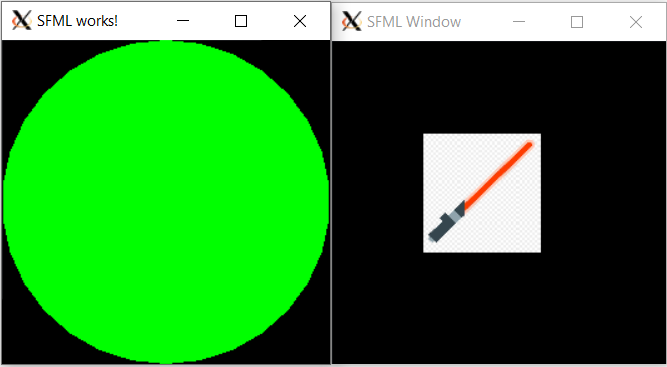
\includegraphics[width=0.5\columnwidth]{ps0_output}
\caption{PS0 Output}
\label{fig:output}
\end{figure}

\subsection{What I Already Knew}\label{sec:ps0:knew} % What was known prior to the assignment

Since this was an intro project, I only had my past C++ coding experience.

\subsection{Design Decisions and Implementations}\label{sec:ps0:decisions} % Important decisions or implementations I made

There were not many major decisions for this project as ti was a demo to learn SFML.
However, since I chose a lightsaber, I thought it was best that a noise to go along with the movement so I chose to do such.

\subsection{What I Learned}\label{sec:ps0:learned} % What I learned because of the assignment

I learned how to run a basic SFML program.
This included generating a window and drawing a sprite to that window.
I learned how to move a sprite using keystrokes which in turn could cause an action, in this cause making a noise.

\subsection{Challenges}\label{sec:ps0:challenges} % Challenges along the way and any that went unresolved

There were were no major complications along the way.

\newpage
\subsection{Codebase}\label{sec:ps0:code} % Code: Makefile, .cpp main, .hpp main, .cpp support, .hpp support, .cpp tests

\bigskip
\title{\large Makefile:}
\lstinputlisting{../ps0/Makefile}
\bigskip
\title{\large main.cpp:}
\lstinputlisting{../ps0/main.cpp}